% This is a sample LaTeX input file.  (Version of 12 August 2004.)
%
% A '%' character causes TeX to ignore all remaining text on the line,
% and is used for comments like this one.

\documentclass{article}      % Specifies the document class

                             % The preamble begins here.
\title{\bf Principles of Computer Systems Design\\ {\Large Assignment 4}}  % Declares the document's title.
\author{Tudor Dragan\\
Sokratis Siozos - Drosos}      % Declares the author's name.
\date{December 16, 2014}      % Deleting this command produces today's date.

\usepackage{verbatimbox}
\usepackage{listings}
\usepackage{color}
\usepackage[]{amsmath}
\usepackage[english]{babel}
\usepackage[utf8]{inputenc}
\usepackage{graphicx}
\usepackage{moreverb}
\usepackage{hyperref}
\usepackage[T1]{fontenc} % font
\usepackage{program}
\usepackage[top=1.5in, bottom=1.5in, left=1.4in, right=1.4in]{geometry}
\usepackage[super]{nth}

\definecolor{dkgreen}{rgb}{0,0.6,0}
\definecolor{gray}{rgb}{0.5,0.5,0.5}
\definecolor{mauve}{rgb}{0.58,0,0.82}

\lstset{frame=tb,
      language=Java,
      aboveskip=3mm,
      belowskip=3mm,
      showstringspaces=false,
      columns=flexible,
      basicstyle={\small\ttfamily},
      numbers=none,
      numberstyle=\tiny\color{gray},
      keywordstyle=\color{blue},
      commentstyle=\color{dkgreen},
      stringstyle=\color{mauve},
      breakatwhitespace=true
      tabsize=3
}
\newcommand{\ip}[2]{(#1, #2)}
                             % Defines \ip{arg1}{arg2} to mean
                             % (arg1, arg2).

%\newcommand{\ip}[2]{\langle #1 | #2\rangle}
                             % This is an alternative definition of
                             % \ip that is commented out.

\begin{document}             % End of preamble and beginning of text.

\maketitle                   % Produces the title.

\section*{Question 1: Reliability} 

Assuming that each node always works, then we only need to consider the probability of failure for each link. Also we assume that each link connects the nodes both ways.\\

We assume that this is a mesh network, and each building directly connects to another building. Finally, a building cannot communicate with a different building through another one because it would end up as a daisy chain network.\\

\begin{enumerate}
\item  
Daisy Chain: 
\begin{equation}
(1-p)^2
\end{equation}

\item  
Fully Connected:
\begin{equation}
(1-p)^3
\end{equation}

\item 
\begin{equation}
(1-0.000001)^2 > (1-0.0001)^3
\end{equation}
So we will pick the daisy chain network because it has a higher probability of all links working correctly.
\end{enumerate}

\section*{Question 2: Distributed Coordination}

According to the theory, the two-phase commit protocol can cause considerable delays to participants in the uncertain state. These delays occur when the coordinator has failed and cannot reply to getDecision requests from participants. Even if a cooperative protocol allows participants to make \emph{getDecision} requests to other participants, delays will occur if the active participants are uncertain.  \\

The Three-phase commit protocol\footnote{\url{http://www.wikiwand.com/en/Three-phase_commit_protocol}} has been designed to alleviate such delays. They are more expensive in the number of messages and the number of rounds required for the normal (failure) case. Specifically, if the timeout of the coordinator occurs after the \emph{preCommit} message, it would send an abort message to all the cohorts. On the Cohort side, since the \emph{preCommit} message has been received, we know that all the other cohorts responded with yes. As a result, if the cohort does not receive a \emph{doCommit} message from the coordinator and the waiting time expires, it will commit and send a \emph{haveCommitted} message back to the coordinator. This way, delays to the participants are avoided.\\ 


\begin{figure}[ht]
\centering
 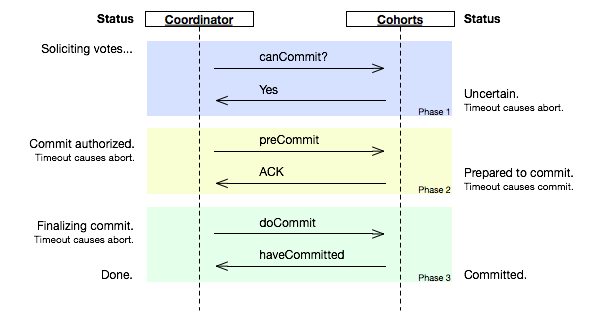
\includegraphics[scale=.5]{img/Three-phase_commit_diagram}
\caption{Three-phase commit protocol \label{overflow}}
\end{figure}

\section*{Programming Task}
\subsection*{Questions for Discussion on the Replication mechanism}

%question 1
In our implementation we decided to use Queue for load balancing. When we get the replicated address in he StockManager proxy and BookStore proxy we take a replicated store address from the beginning of the quest and add it again. This way we ensure that the load is balanced evenly through the replicated stores.\\

\begin{figure}[htbp]
\begin{center}
\begin{lstlisting}
public String getReplicaAddress() {
		String address = loadBalanceQueue.poll();
		loadBalanceQueue.add(address);
		return address;
	}
\end{lstlisting}
\caption{getReplicaAddress method}
\label{getReplicaAddress method}
\end{center}
\end{figure}

The latency hiding is achieved by not having to wait for the replication process to finish. We do this by sending the replication request to the slave servers and constructing a list of Future objects. A Future represents the result of an asynchronous computation. Methods are provided to check if the computation is complete, to wait for its completion, and to retrieve the result of the computation. \\ 

Fail-stop subsystems require that the higher-level subsystem take some additional measure to discover the failure, for example by setting a timer and responding to its expiration. A problem with fail-stop design is that it can be difficult to distinguish a stopped subsystem from one that is merely running more slowly than expected. This problem is particularly acute in asynchronous systems.\footnote{Principles of Computer System Design (PCSD) - DIKU Course Compendium, p.251, 2013/2014} The waitForSlaveUpdates method in the MasterCertainBookStore class actually handles the failed slaves by analyzing their response and removing them from the list when necessary, thus implementing a fail-stop model. \\ 

The Replicator is basically an HttpClient that sends replication requests  from the Master Server to the Slave Servers. We used an ExecutorService for handling the asynchronous communication and by adding tasks to its thread pool of executors.\\

\begin{figure}[htbp]
\begin{center}
\begin{lstlisting}
CertainBookStoreReplicationTask task = 
	new CertainBookStoreReplicationTask(server, request, replicationClient);
results.add(executorService.submit(task));
\end{lstlisting}
\caption{Adding a Task to the Executor Service}
\label{Adding a Task to the Executor Service}
\end{center}
\end{figure}



\end{document}               % End of document.